%%%%%%%%%%%%%%%%%%%%%%%%%%%%%%%%%%%%%%%%%%%%%%%%%%%%%%%
% MatPlotLib and Random Cheat Sheet
%
% Edited by Maverick Lin
%
%%%%%%%%%%%%%%%%%%%%%%%%%%%%%%%%%%%%%%%%%%%%%%%%%%%%%%%

% \documentclass{article}
\documentclass[9pt]{extarticle}
\usepackage[landscape]{geometry}
\usepackage{url}
\usepackage{multicol}
\usepackage{amsmath}
\usepackage{amsfonts}
\usepackage{tikz}
\usetikzlibrary{decorations.pathmorphing}
\usepackage{amsmath,amssymb}
\usepackage{tabularx}

\usepackage{colortbl}
\usepackage{xcolor}
\usepackage{mathtools}
\usepackage{amsmath,amssymb}
\usepackage{enumitem}
\usepackage{tabto}
\usepackage{enumitem}
\usepackage{graphicx}
\usepackage{tabu}

\title{Google Data Engineer Notes}
\usepackage[brazilian]{babel}
\usepackage[utf8]{inputenc}

\advance\topmargin-.8in
\advance\textheight3in
\advance\textwidth3in
\advance\oddsidemargin-1.5in
\advance\evensidemargin-1.5in
\parindent0pt
\parskip2pt
\newcommand{\hr}{\centerline{\rule{3.5in}{1pt}}}
%\colorbox[HTML]{e4e4e4}{\makebox[\textwidth-2\fboxsep][l]{texto}
\begin{document}

\begin{center}{\huge{\textbf{Google Data Engineering Cheatsheet}}}\\
{\large Compiled by Maverick Lin (\url{http://mavericklin.com})}\\
{\normalsize Last Updated August 4, 2018}
\end{center}
\begin{multicols*}{3}

\tikzstyle{mybox} = [draw=black, fill=white, very thick, rectangle, rounded corners, inner sep=10pt, inner ysep=10pt]
\tikzstyle{fancytitle} =[fill=black, text=white, font=\bfseries]


%------------ What is Data Engineering? ---------------
\begin{tikzpicture}
\node [mybox] (box){%
    \begin{minipage}{0.3\textwidth}
	Data engineering enables data-driven decision making by collecting, transforming, and visualizing data. A data engineer designs, builds, maintains, and troubleshoots data processing systems with a particular emphasis on the security, reliability, fault-tolerance, scalability, fidelity, and efficiency of such systems.\\

	A data engineer also analyzes data to gain insight into business outcomes, builds statistical models to support decision-making, and creates machine learning models to automate and simplify key business processes. \\
        
	Key Points
    \setlist{nolistsep}	
    \begin{itemize}
    	\item Build/maintain data structures and databases
		\item Design data processing systems
        \item Analyze data and enable machine learning
        \item Design for reliability
        \item Visualize data and advocate policy
        \item Model business processes for analysis
        \item Design for security and compliance
    \end{itemize}
    
    \end{minipage}
};
\node[fancytitle, right=10pt] at (box.north west) {What is Data Engineering?};
\end{tikzpicture}


%------------ Google Compute Platform (GCP) ---------------
\begin{tikzpicture}
\node [mybox] (box){%
    \begin{minipage}{0.3\textwidth}
		GCP is a collection of Google computing resources, which are offered via \textit{services}. Data engineering services include Compute, Storage, Big Data, and Machine Learning.\\
        
        The 4 ways to interact with GCP include the console, command-line-interface (CLI), API, and mobile app.\\

        The GCP resource hierarchy is organized as follows. All resources (VMs, storage buckets, etc) are organized into \textbf{projects}. These projects \textit{may} be organized into \textbf{folders}, which can contain other folders. All folders and projects can be brought together under an organization node. Project folders and organization nodes are where policies can be defined. Policies are inherited downstream and dictate who can access what resources. Every resource must belong to a project and every must have a billing account associated with it.\\
        
    \textbf{Advantages}: Performance (fast solutions), Pricing (sub-hour billing, sustained use discounts, custom machine types), PaaS Solutions, Robust Infrastructure
    \end{minipage};

};
\node[fancytitle, right=10pt] at (box.north west) {Google Compute Platform (GCP)};
\end{tikzpicture}


%------------ Hadoop Overview ---------------
\begin{tikzpicture}
\node [mybox] (box){%
    \begin{minipage}{0.3\textwidth}
    \setlist{nolistsep}	

    {\color{blue} \textbf{Hadoop}}\\
    Data can no longer fit in memory on one machine (monolithic), so a new way of computing was devised using many computers to process the data (distributed). Such a group is called a cluster, which makes up server farms. All of these servers have to be coordinated in the following ways: partition data, coordinate computing tasks, handle fault tolerance/recovery, and allocate capacity to process.\\
    
    Hadoop is an open source \textit{distributed} processing framework that manages data processing and storage for big data applications running in clustered systems. It is comprised of 3 main components:
    \begin{itemize}
    	\item \textbf{Hadoop Distributed File System (HDFS)}: a distributed file system that provides high-throughput access to application data by partitioning data across many machines
        \item \textbf{YARN}: framework for job scheduling and cluster resource management (task coordination)
        \item \textbf{MapReduce}: YARN-based system for parallel processing of large data sets on multiple machines\\
	\end{itemize}

    {\color{blue} \textbf{HDFS}}\\
    Each disk on a different machine in a cluster is comprised of 1 master node; the rest are data nodes. The \textbf{master node} manages the overall file system by storing the directory structure and metadata of the files. The \textbf{data nodes} physically store the data. Large files are broken up/distributed across multiple machines, which are replicated across 3 machines to provide fault tolerance.\\
    
   {\color{blue} \textbf{MapReduce}}\\
   Parallel programming paradigm which allows for processing of huge amounts of data by running processes on multiple machines. Defining a MapReduce job requires two stages: map and reduce.
   
   \begin{itemize}
   	\item \textbf{Map}: operation to be performed in parallel on small portions of the dataset. the output is a key-value pair $<K,V>$
    \item \textbf{Reduce}: operation to combine the results of Map\\
   \end{itemize}
   
   {\color{blue} \textbf{YARN- Yet Another Resource Negotiator}}\\
   Coordinates tasks running on the cluster and assigns new nodes in case of failure. Comprised of 2 subcomponents: the resource manager and the node manager. The \textbf{resource manager} runs on  a single master node and schedules tasks across nodes. The \textbf{node manager} runs on all other nodes and manages tasks on the individual node.
    
%     A typical job process: the user defines defines the map and reduce tasks using MapReduce API, the job is triggered on the Hadoop cluster, YARN figures out where and how to run the job and stores the result in HDFS.

    \end{minipage};

};
\node[fancytitle, right=10pt] at (box.north west) {Hadoop Overview};
\end{tikzpicture}





%------------ Hadoop Ecosystem ---------------
\begin{tikzpicture}
\node [mybox] (box){%
    \begin{minipage}{0.3\textwidth}
    An entire ecosystem of tools have emerged around Hadoop, which are based on interacting with HDFS.\\
    
    {\color{cyan} \textbf{Hive}}: data warehouse software built o top of Hadoop that facilitates reading, writing, and managing large datasets residing in distributed storage using SQL-like queries (HiveQL). Hive abstracts away underlying MapReduce jobs and returns HDFS in the form of tables (not HDFS). \\
    {\color{cyan} \textbf{Pig}}: high level scripting language (Pig Latin) that enables writing complex data transformations. It pulls unstructured/incomplete data from sources, cleans it, and places it in a database/data warehouses. Pig performs ETL into data warehouse while Hive queries from data warehouse to perform analysis (GCP: DataFlow).\\
    {\color{cyan} \textbf{Spark}}: framework for writing fast, distributed programs for data processing and analysis. Spark solves similar problems as Hadoop MapReduce but with a fast in-memory approach. It is an unified engine that supports SQL queries, streaming data, machine learning and graph processing. Can operate separately from Hadoop but integrates well with Hadoop. Data is processed using Resilient Distributed Datasets (RDDs), which are immutable, lazily evaluated, and tracks lineage. \\
    {\color{cyan} \textbf{Hbase}}: non-relational, NoSQL, column-oriented database management system that runs on top of HDFS. Well suited for sparse data sets (GCP: BigTable)  \\
    {\color{cyan} \textbf{Flink/Kafka}}: stream processing framework. Batch streaming is for bounded, finite datasets, with periodic updates, and delayed processing. Stream processing is for unbounded datasets, with continuous updates, and immediate processing. Stream data and stream processing must be decoupled via a message queue. Can group streaming data (windows) using tumbling (non-overlapping time), sliding (overlapping time), or session (session gap) windows. \\
    {\color{cyan} \textbf{Beam}}: programming model to define and execute data processing pipelines, including ETL, batch and stream (continuous) processing. After building the pipeline, it is executed by one of Beam’s distributed processing back-ends (Apache Apex, Apache Flink, Apache Spark, and Google Cloud Dataflow). Modeled as a Directed Acyclic Graph (DAG).\\
     {\color{cyan} \textbf{Oozie}}: workflow scheduler system to manage Hadoop jobs\\
     {\color{cyan} \textbf{Sqoop}}: transferring framework to transfer large amounts of data into HDFS from relational databases (MySQL)
    \end{minipage};
};
\node[fancytitle, right=10pt] at (box.north west) {Hadoop Ecosystem};
\end{tikzpicture}


% ------------ IAM -----------------
\begin{tikzpicture}
\node [mybox] (box){%
    \begin{minipage}{0.3\textwidth}
    \setlist{nolistsep}	

    {\color{blue} \textbf{Identity Access Management (IAM)}}\\
    Access management service to manage different members of the platform- who has what access for which resource.\\
    
    Each member has roles and permissions to allow them access to perform their duties on the platform. 3 member types: Google account (single person, gmail account), service account (non-person, application), and Google Group (multiple people). Roles are a set of specific permissions for members. Cannot assign permissions to user directly, must grant roles.\\
    
      If you grant a member access on a higher hierarchy level, that member will have access to all levels below that hierarchy level as well. You cannot be restricted a lower level. The policy is a union of assigned and inherited policies.\\
    
    \textbf{Primitive Roles}: Owner (full access to resources, manage roles), Editor (edit access to resources, change or add), Viewer (read access to resources)\\
    \textbf{Predefined Roles}: finer-grained access control than primitive roles, predefined by Google Cloud\\
    \textbf{Custom Roles}\\
    
    \textbf{Best Practice}: use predefined roles when they exist (over primitive). Follow the principle of least privileged favors.
    

    \end{minipage}
};
\node[fancytitle, right=10pt] at (box.north west) {IAM};
\end{tikzpicture}


% ------------ Stackdriver -----------------
\begin{tikzpicture}
\node [mybox] (box){%
    \begin{minipage}{0.3\textwidth}
    \setlist{nolistsep}	
    GCP's monitoring, logging, and diagnostics solution. Provides insights to health, performance, and availability of applications.\\
    Main Functions
    \begin{itemize}
    	\item \textbf{Debugger}: inspect state of app in real time without stopping/slowing down e.g. code behavior
        \item \textbf{Error Reporting}: counts, analyzes, aggregates crashes in cloud services
    	\item \textbf{Monitoring}: overview of performance, uptime and heath of cloud services (metrics, events, metadata)
    	\item \textbf{Alerting}: create policies to notify you when health and uptime check results exceed a certain limit
    	\item \textbf{Tracing}: tracks how requests propagate through applications/receive near real-time performance results, latency reports of VMs
        \item \textbf{Logging}: store, search, monitor and analyze log data and events from GCP

	\end{itemize}
    \end{minipage}
};
\node[fancytitle, right=10pt] at (box.north west) {Stackdriver};
\end{tikzpicture}


% ------------ Key Concepts -----------------
\begin{tikzpicture}
\node [mybox] (box){%
    \begin{minipage}{0.3\textwidth}
    \setlist{nolistsep}	

    
    {\color{blue} \textbf{OLAP vs. OLTP}}\\
    \textbf{Online Analytical Processing (OLAP)}: primary objective is data analysis. It is an online analysis and data retrieving process, characterized by a large volume of data and complex queries, uses data warehouses.\\
    \textbf{Online Transaction Processing (OLTP)}: primary objective is data processing, manages database modification, characterized by large numbers of short online transactions, simple queries, and traditional DBMS.\\
    
    {\color{blue} \textbf{Row vs. Columnar Database}}\\
    \textbf{Row Format}: stores data by row\\
	\textbf{Column Format}: stores data tables by column rather than by row, which is suitable for analytical query processing and data warehouses\\
    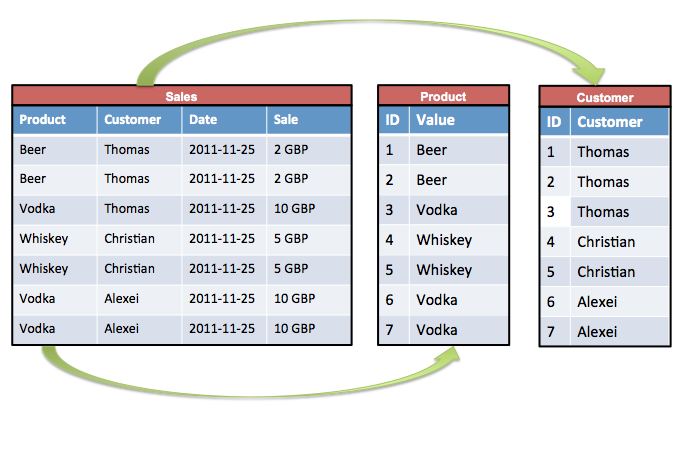
\includegraphics[width=\textwidth, height=4cm]{Figures/column.png}
    
    {\color{blue} \textbf{IaaS, Paas, SaaS}}\\
    \textbf{IaaS}: gives you the infrastructure pieces (VMs) but you have to maintain/join together the different infrastructure pieces for your application to work. Most flexible option.\\
    \textbf{PaaS}: gives you all the infrastructure pieces already joined so you just have to deploy source code on the platform for your application to work. PaaS solutions are managed services/no-ops (highly available/reliable) and serverless/autoscaling (elastic). Less flexible than IaaS\\

    
    {\color{blue} \textbf{Fully Managed, Hotspotting}}
    
    \end{minipage}
};
\node[fancytitle, right=10pt] at (box.north west) {Key Concepts};
\end{tikzpicture}


% ------------ Compute Choices -----------------
\begin{tikzpicture}
\node [mybox] (box){%
    \begin{minipage}{0.3\textwidth}
    
    {\color{blue} \textbf{Google App Engine}}\\
    Flexible, serverless platform for building highly available applications. Ideal when you want to focus on writing and developing code and do not want to manage servers, clusters, or infrastructures. \\
    \textbf{Use Cases:} web sites, mobile app and gaming backends, RESTful APIs, IoT apps.\\
    
    {\color{blue} \textbf{Google Kubernetes (Container) Engine}}\\
    Logical infrastructure powered by Kubernetes, an open-source container orchestration system. Ideal for managing containers in production, increase velocity and operatability, and don't have OS dependencies.\\
    \textbf{Use Cases:} containerized workloads, cloud-native distributed systems, hybrid applications.\\
    
    {\color{blue} \textbf{Google Compute Engine} (IaaS)}\\
    Virtual Machines (VMs) running in Google's global data center. Ideal for when you need complete control over your infrastructure and direct access to high-performance hardward or need OS-level changes.\\
    \textbf{Use Cases:} any workload requiring a specific OS or OS configuration, currently deployed and on-premises software that you want to run in the cloud.\\
    
    \textbf{Summary}: AppEngine is the PaaS option- serverless and ops free. ComputeEngine is the IaaS option- fully controllable down to OS level. Kubernetes Engine is in the middle- clusters of machines running Kuberenetes and hosting containers. 
    
    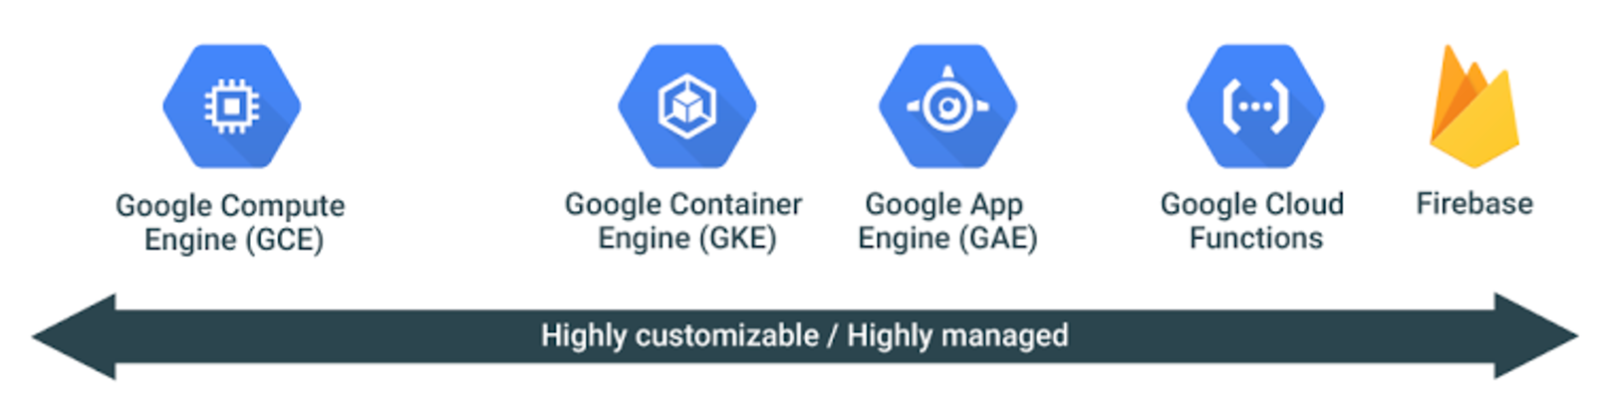
\includegraphics[width=\textwidth]{Figures/Compute.png}
    
    {\color{blue} \textbf{Additional Notes}}\\
    You can also mix and match multiple compute options.\\
    \textbf{Preemptible Instances}: instances that run at a much lower price but may be terminated at any time, self-terminate after 24 hours. ideal for interruptible workloads\\
    \textbf{Snapshots}: used for backups of disks\\
    \textbf{Images}: VM OS (Ubuntu, CentOS)
    \setlist{nolistsep}	
    \end{minipage}
};
\node[fancytitle, right=10pt] at (box.north west) {Compute Choices};
\end{tikzpicture}



% ------------ Storage Options -----------------
\begin{tikzpicture}
\node [mybox] (box){%
    \begin{minipage}{0.3\textwidth}
    \setlist{nolistsep}	

    {\color{blue} \textbf{Persistent Disk}} Fully-managed block storage (SSDs) that is suitable for VMs/containers. Good for snapshots of data backups/sharing read-only data across VMs.\\
    
    {\color{blue} \textbf{Cloud Storage}} Infinitely scalable, fully-managed and highly reliable object/blob storage. Good for data blobs: images, pictures, videos. Cannot query by content.\\
    
    To use Cloud Storage, you create buckets to store data and the location can be specified. Bucket names are globally unique. There a 4 storage classes:
    \begin{itemize}
        \item \textbf{Multi-Regional}: frequent access from anywhere in the world. Use for "hot data"
        \item \textbf{Regional}: high local performance for region
        \item \textbf{Nearline}: storage for data accessed less than once a month (archival)
        \item \textbf{Coldline}: less than once a year (archival)
    \end{itemize}

    \end{minipage}
};
\node[fancytitle, right=10pt] at (box.north west) {Storage};
\end{tikzpicture}


% % ------------ Storage- Database Options -----------------
% \begin{tikzpicture}
% \node [mybox] (box){%
%     \begin{minipage}{0.3\textwidth}
%     \setlist{nolistsep}	
    
%     Non-relational databases holds non-relational data, or data that doesn't have a fixed structure . Think documents, hierarchical data, key-value attributes, graph data, etc...\\
   
%     {\color{blue} \textbf{BigTable}} Scalable, fully-managed NoSQL wide-column database. Good for real-time access and analytics workloads, low-latency read/write access, high-throughput analytics, and native time series support. Sensitive to hot-spotting.\\
    
%     {\color{blue} \textbf{Datastore}} Scalable, fully-managed NoSQL document database for web and mobile applications. Good for semi-structured application data, hierarchical data, ad durable key-value data.
    
%     \end{minipage}
% };
% \node[fancytitle, right=10pt] at (box.north west) {Storage- Non-Relational Databases};
% \end{tikzpicture}



% ------------ CloudSQL and Cloud Spanner -----------------
\begin{tikzpicture}
\node [mybox] (box){%
    \begin{minipage}{0.3\textwidth}
    \setlist{nolistsep}	

    
    {\color{blue} \textbf{Cloud SQL}} \\
    Fully-managed relational database service (supports MySQL/PostgreSQL). Use for relational data: tables, rows and columns, and super structured data. SQL compatible and can update fields. Not scalable (small storage- GBs). Good for web frameworks and OLTP workloads (not OLAP). Can use \textbf{Cloud Storage Transfer Service} or \textbf{Transfer Appliance} to data into Cloud Storage (from AWS, local, another bucket). Use gsutil if copying files over from on-premise.\\
    
    {\color{blue} \textbf{Cloud Spanner}} \\
    Google-proprietary offering, more advanced than Cloud SQL. Mission-critical, relational database. Supports horizontal scaling. Combines benefits of of relational and non-relational databases.
    
    \begin{itemize}
    	\item \textbf{Ideal}: relational, structured, and semi-structured data that requires high availability, strong consistency, and transactional reads and writes
        \item \textbf{Avoid}: data is not relational or structured, want an open source RDBMS, strong consistency and high availability is unnecessary\\
    \end{itemize}
    
    {\color{cyan} \textbf{Cloud Spanner Data Model}} \\
    A database can contain 1+ tables. Tables look like relational database tables. Data is strongly typed: must define a schema for each database and that schema must specify the data types of each column of each table.  \\
    \textbf{Parent-Child Relationships}: Can optionally define relationships between tables to physically co-locate their rows for efficient retrieval (data locality: physically storing 1+ rows of a table with a row from another table.

    \end{minipage}
};
\node[fancytitle, right=10pt] at (box.north west) {CloudSQL and Cloud Spanner- Relational DBs};
\end{tikzpicture}

% ------------ BigTable -----------------
\begin{tikzpicture}
\node [mybox] (box){%
    \begin{minipage}{0.3\textwidth}
    \setlist{nolistsep}	
    
    Columnar database ideal applications that need high throughput, low latencies, and scalability (IoT, user analytics, time-series data, graph data) for non-structured key/value data (each value is $<$ 10 MB). A single value in each row is indexed and this value is known as the row key. Does not support SQL queries. Zonal service. Not good for data less than 1TB of data or items greater than 10MB. Ideal at handling large amounts of data (TB/PB) for long periods of time.\\

    {\color{blue} \textbf{Data Model}}\\
    4-Dimensional: row key, column family (table name), column name, timestamp.
   	\begin{itemize}
    \item Row key uniquely identifies an entity and columns contain individual values for each row. 
    \item Similar columns are grouped into column families.  
    \item Each column is identified by a combination of the column family and a column qualifier, which is a unique name within the column family.
    \end{itemize}
    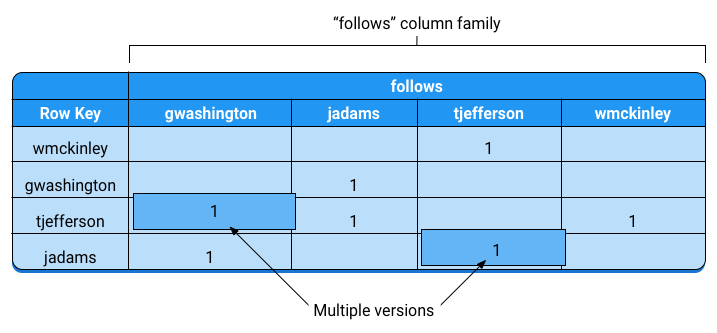
\includegraphics[width=\textwidth]{Figures/bigtable-example.png}
    
    {\color{blue} \textbf{Load Balancing}}
    Automatically manages splitting, merging, and rebalancing. The master process balances workload/data volume within clusters. The master splits busier/larger tablets in half and merges less-accessed/smaller tablets together, redistributing them between nodes. \\
    Best write performance can be achieved by using row keys that do not follow a predictable order and grouping related rows so they are adjacent to one another, which results in more efficient multiple row reads at the same time.\\
    
    {\color{blue} \textbf{Security}}
    Security can be managed at the project and instance level. Does not support table-level, row-level, column-level, or cell-level security restrictions.\\


    
    {\color{blue} \textbf{Other Storage Options}}\\
    - Need SQL for OLTP: CloudSQL/Cloud Spanner.\\
    - Need interactive querying for OLAP: BigQuery.\\
    - Need to store blobs larger than 10 MB: Cloud Storage.\\
    - Need to store structured objects in a document database, with ACID and SQL-like queries: Cloud Datastore.
    \end{minipage}
};
\node[fancytitle, right=10pt] at (box.north west) {BigTable};
\end{tikzpicture}


% ------------ BigTable Part II -----------------
\begin{tikzpicture}
\node [mybox] (box){%
    \begin{minipage}{0.3\textwidth}
    \setlist{nolistsep}	
    
    {\color{blue} \textbf{Designing Your Schema}}\\
    Designing a Bigtable schema is different than designing a schema for a RDMS. Important considerations:
    \begin{itemize}
    	\item Each table has only one index, the row key (4 KB)
        \item Rows are \textbf{sorted lexicographically by row key}.
        \item All operations are \textbf{atomic} (ACID) at row level.
        \item Both reads and writes should be distributed evenly
        \item Try to keep all info for an entity in a single row
        \item Related entities should be stored in adjacent rows
        \item Try to store \textbf{10 MB in a single cell} (max 100 MB) and \textbf{100 MB in a single row} (256 MB)
        \item Supports max of 1,000 tables in each instance.
        \item Choose row keys that don't follow predictable order
        \item Can use up to around 100 column families
        \item Column Qualifiers: can create as many as you need in each row, but should avoid splitting data across more column qualifiers than necessary (16 KB)
        \item \textbf{Tables are sparse}. Empty columns don't take up any space. Can create large number of columns, even if most columns are empty in most rows.
        \item Field promotion (shift a column as part of the row key) and salting (remainder of division of hash of timestamp plus row key) are ways to help design row keys.\\
        
        \end{itemize}

    
    For time-series data, use tall/narrow tables.\\
    Denormalize- prefer multiple tall and narrow tables
       

    \end{minipage}
};
\node[fancytitle, right=10pt] at (box.north west) {BigTable Part II};
\end{tikzpicture}




% ------------ BigQuery -----------------
\begin{tikzpicture}
\node [mybox] (box){%
    \begin{minipage}{0.3\textwidth}
    \setlist{nolistsep}	
       Scalable, fully-managed Data Warehouse with extremely fast SQL queries. Allows querying for massive volumes of data at fast speeds. Good for OLAP workloads (petabyte-scale), Big Data exploration and processing, and reporting via Business Intelligence (BI) tools. Supports SQL querying for non-relational data. Relatively cheap to store, but costly for querying/processing. Good for analyzing historical data.\\
       
       {\color{blue} \textbf{Data Model}} \\
		Data tables are organized into units called datasets, which are sets of tables and views. A table must belong to dataset and a datatset must belong to a porject. Tables contain records with rows and columns (fields).
       
       You can load data into BigQuery via two options: batch loading (free) and streaming (costly).\\
       
       {\color{blue} \textbf{Security}} \\
       BigQuery uses IAM to manage access to resources. The three types of resources in BigQuery are organizations, projects, and datasets. Security can be applied at the project and dataset level, but not table or view level. \\
%        Project-level access controls determine the users, groups, and service accounts allowed to access all datasets, tables, views, and table data within a project. Dataset-level access controls determine the users, groups, and service accounts allowed to access the tables, views, and table data in a specific dataset.\\
       
       {\color{blue} \textbf{Views}} \\
       A view is a virtual table defined by a SQL query. When you create a view, you query it in the same way you query a table. \textbf{Authorized views allow you to share query results with particular users/groups without giving them access to underlying data.} When a user queries the view, the query results contain data only from the tables and fields specified in the query that defines the view.\\
       
       {\color{blue} \textbf{Billing}} \\
       Billing is based on \textbf{storage} (amount of data stored), \textbf{querying} (amount of data/number of bytes processed by query), and \textbf{streaming inserts}. Storage options are active and long-term (modified or not past 90 days). Query options are on-demand and flat-rate. \\
       Query costs are based on how much data you read/process, so if you only read a section of a table (partition), your costs will be reduced. Any charges occurred are billed to the attached billing account. Exporting/importing/copying data is free.
       


    \end{minipage}
};
\node[fancytitle, right=10pt] at (box.north west) {BigQuery};
\end{tikzpicture}


% ------------ BigQuery Part II -----------------
\begin{tikzpicture}
\node [mybox] (box){%
    \begin{minipage}{0.3\textwidth}
    \setlist{nolistsep}	
    	
    {\color{blue} \textbf{Partitioned tables}}\\
    Special tables that are divided into partitions based on a column or partition key. Data is stored on different directories and specific queries will only run on slices of data, which improves query performance and reduces costs. Note that the partitions will not be of the same size. BigQuery automatically does this.\\
    Each partitioned table can have up to 2,500 partitions (2500 days or a few years). The daily limit is 2,000 partition updates per  table, per day. The rate limit: 50 partition updates every 10 seconds.\\
    
    Two types of partitioned tables:
    \begin{itemize}
    	\item \textbf{Ingestion Time}: Tables partitioned based on the data's ingestion (load) date or arrival date. Each partitioned table will have  pseudocolumn \_PARTITIONTIME, or time data was loaded into table. Pseudocolumns are reserved for the table and cannot be used by the user. 
		\item \textbf{Partitioned Tables}: Tables that are partitioned based on a TIMESTAMP or DATE column.\\
	\end{itemize}
    
    \textbf{Windowing}: window functions increase the efficiency and reduce the complexity of queries that analyze partitions (windows) of a dataset by providing complex operations without the need for many intermediate calculations. They reduce the need for intermediate tables to store temporary data\\
    
    {\color{blue} \textbf{Bucketing}}\\
    Like partitioning, but each split/partition should be the same size and is based on the hash function of a column. Each bucket is a separate file, which makes for more efficient sampling and joining data.\\
    

    
    {\color{blue} \textbf{Querying}}\\
    After loading data into BigQuery, you can query using Standard SQL (preferred) or Legacy SQL (old). Query jobs are actions executed asynchronously to load, export, query, or copy data. Results can be saved to permanent (store) or temporary (cache) tables. 2 types of queries:
    \begin{itemize}
    	\item \textbf{Interactive}: query is executed immediately, counts toward daily/concurrent usage (default)
		\item \textbf{Batch}: batches of queries are queued and the query starts when idle resources are available, only counts for daily and switches to interactive if idle for 24 hours\\
	\end{itemize}

    {\color{blue} \textbf{Wildcard Tables}}\\
    Used if you want to union all similar tables with similar names. '*' (e.g. project.dataset.Table*)

    
    
    
    
    \end{minipage}
};
\node[fancytitle, right=10pt] at (box.north west) {BigQuery Part II};
\end{tikzpicture}

% ------------ Optimizing BigQuery -----------------
\begin{tikzpicture}
\node [mybox] (box){%
    \begin{minipage}{0.3\textwidth}
    \setlist{nolistsep}	

    
    {\color{blue} \textbf{Controlling Costs}}\\
    - Avoid SELECT * (full scan), select only columns needed (SELECT * EXCEPT)\\
    - Sample data using preview options for free\\
    - Preview queries to estimate costs (dryrun) \\
    - Use max bytes billed to limit query costs\\
    - Don't use LIMIT clause to limit costs (still full scan)\\
    - Monitor costs using dashboards and audit logs\\
    - Partition data by date\\
    - Break query results into stages\\
    - Use default table expiration to delete unneeded data\\
    - Use streaming inserts wisely\\
    - Set hard limit on bytes (members) processed per day\\
    
    {\color{blue} \textbf{Query Performance}}\\
    Generally, queries that do less work perform better.\\
    
    \textbf{Input Data/Data Sources}\\
    - Avoid SELECT * \\
    - Prune partitioned queries (for time-partitioned table, use PARTITIONTIME pseudo column to filter partitions)\\
    - Denormalize data (use nested and repeated fields)\\
    - Use external data sources appropriately\\
    - Avoid excessive wildcard tables\\
    
    \textbf{SQL Anti-Patterns}\\
    - Avoid self-joins., use window functions (perform calculations across many table rows related to current row)\\
    - Partition/Skew: avoid unequally sized partitions, or when a value occurs more often than any other value\\
    - Cross-Join: avoid joins that generate more outputs than inputs (pre-aggregate data or use window function)\\
    Update/Insert Single Row/Column: avoid point-specific DML, instead batch updates and inserts\\
    
    \textbf{Managing Query Outputs}\\
    - Avoid repeated joins and using the same subqueries\\
    - Writing large sets has performance/cost impacts. Use filters or LIMIT clause. 128MB limit for cached results\\
    - Use LIMIT clause for large sorts (Resources Exceeded)\\
    
    \textbf{Optimizing Query Computation}\\
    - Avoid repeatedly transforming data via SQL queries\\
    - Avoid JavaScript user-defined functions\\
    - Use approximate aggregation functions (approx count)\\
    - Order query operations to maximize performance. Use ORDER BY only in outermost query, push complex operations to end of the query.\\
    - For queries that join data from multiple tables, optimize join patterns. Start with the largest table.    
    \end{minipage}
};
\node[fancytitle, right=10pt] at (box.north west) {Optimizing BigQuery};
\end{tikzpicture}




% ------------ DataStore -----------------
\begin{tikzpicture}
\node [mybox] (box){%
    \begin{minipage}{0.3\textwidth}
    \setlist{nolistsep}	
	NoSQL document database that automatically handles sharding and replication (highly available, scalable and durable). Supports ACID transactions, SQL-like queries. Query execution depends on size of returned result, not size of dataset. Ideal for "needle in a haystack" operation and applications that rely on highly available structured data at scale\\
    
    {\color{blue} \textbf{Data Model}}\\
    Data objects in Datastore are known as entities. An entity has one or more named properties, each of which can have one or more values. Each entity in has a key that uniquely identifies it. You can fetch an individual entity using the entity's key, or query one or more entities based on the entities' keys or property values.\\
    
    Ideal for highly structured data at scale: product catalogs, customer experience based on users past activities/preferences, game states. Don't use if you need extremely low latency or analytics (complex joins, etc).\\

    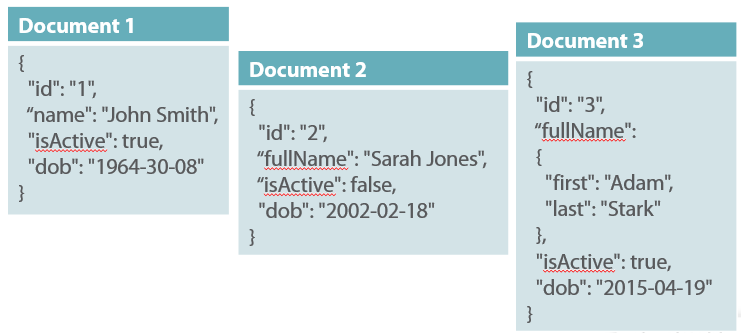
\includegraphics[width=\textwidth]{Figures/DocumentDatabase.png}

    \end{minipage}
};
\node[fancytitle, right=10pt] at (box.north west) {DataStore};
\end{tikzpicture}

% ------------ DataProc -----------------
\begin{tikzpicture}
\node [mybox] (box){%
    \begin{minipage}{0.3\textwidth}
    \setlist{nolistsep}	
    
    Fully-managed cloud service for running Spark and Hadoop clusters. Provides access to Hadoop cluster on GCP and Hadoop-ecosystem tools (Pig, Hive, and Spark). Can be used to implement ETL warehouse solution.\\
    
    Preferred if migrating existing on-premise Hadoop or Spark infrastructure to GCP without redevelopment effort. Dataflow is preferred for a new development.
    \end{minipage}
};
\node[fancytitle, right=10pt] at (box.north west) {DataProc};
\end{tikzpicture}

% ------------ DataFlow -----------------
\begin{tikzpicture}
\node [mybox] (box){%
    \begin{minipage}{0.3\textwidth}
    \setlist{nolistsep}	
    
    Managed service for developing and executing data processing patterns (ETL) (based on Apache Beam) for \textbf{streaming} and \textbf{batch} data. Preferred for new Hadoop or Spark infrastructure development. Usually site between front-end and back-end storage solutions. \\

    {\color{blue} \textbf{Concepts}}\\
    \textbf{Pipeline}: encapsulates series of computations that accepts input data from external sources, transforms data to provide some useful intelligence, and produce output\\
    \textbf{PCollections}: abstraction that represents a potentially distributed, multi-element data set, that acts as the pipeline's data. PCollection objects represent input, intermediate, and output data. The edges of the pipeline.\\
    \textbf{Transforms}: operations in pipeline. A transform takes a PCollection(s) as input, performs an operation that you specify on each element in that collection, and produces a new output PCollection. Uses the "what/where/when/how" model. Nodes in the pipeline. Composite transforms are multiple transforms: combining, mapping, shuffling, reducing, or statistical analysis.\\
    \textbf{Pipeline I/O}: the source/sink, where the data flows in and out. Supports read and write transforms for a number of common data storage types, as well as custom.\\
    
    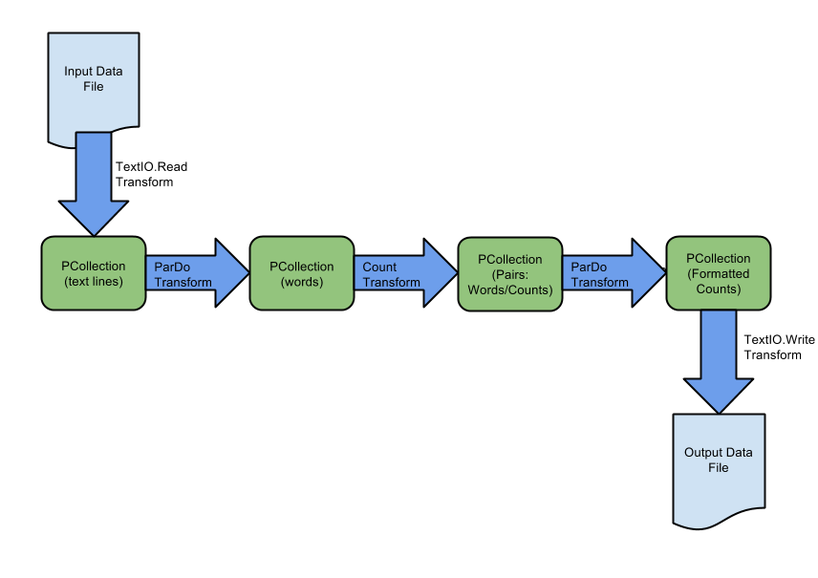
\includegraphics[width=\textwidth]{Figures/beam_pipeline.png}
    
    {\color{blue} \textbf{Windowing}}\\
    Windowing a PCollection divides the elements into windows based on the associated event time for each element. Especially useful for PCollections with unbounded size, since it allows operating on a sub-group (mini-batches).\\
    
    {\color{blue} \textbf{Triggers}}\\
    Allows specifying a trigger to control when (in processing time) results for the given window can be produced. If unspecified, the default behavior is to trigger first when the watermark passes the end of the window, and then trigger again every time there is late arriving data.
    
    \end{minipage}
};
\node[fancytitle, right=10pt] at (box.north west) {DataFlow};
\end{tikzpicture}

% ------------ Pub/Sub -----------------
\begin{tikzpicture}
\node [mybox] (box){%
    \begin{minipage}{0.3\textwidth}
    \setlist{nolistsep}	
    
    Asynchronous messaging service that decouples senders and receivers. Allows for secure and highly available communication between independently written applications. \\
    A publisher app creates and sends messages to a \textit{topic}. Subscriber applications create a subscription to a topic to receive messages from it. Communication can be one-to-many (fan-out), many-to-one (fan-in), and many-to-many. Gaurantees at least once delivery before deletion from queue.\\
    
    {\color{blue} \textbf{Scenarios}}
    \begin{itemize}
    	\item Balancing workloads in network clusters- queue can efficiently distribute tasks
       	\item Implementing asynchronous workflows
        \item Data streaming from various processes or devices
        \item Reliability improvement- in case zone failure
         \item Distributing event notifications
        \item Refreshing distributed caches
        \item Logging to multiple systems\\
	\end{itemize}
    
    
    {\color{blue} \textbf{Benefits/Features}}\\
    Unified messaging, global presence, push- and pull-style subscriptions,  replicated storage and guaranteed at-least-once message delivery, encryption of data at rest/transit, easy-to-use REST/JSON API\\
        
     {\color{blue} \textbf{Data Model}}\\
     \textbf{Topic}, \textbf{Subscription}, \textbf{Message} (combination of data and attributes that a publisher sends to a topic and is eventually delivered to subscribers), \textbf{Message Attribute} (key-value pair that a publisher can define for a message)\\
     
     {\color{blue} \textbf{Message Flow}}
     \begin{itemize}
     	\item Publisher creates a topic in the Cloud Pub/Sub service and sends messages to the topic.
		\item Messages are persisted in a message store until they are delivered and acknowledged by subscribers.
		\item The Pub/Sub service forwards messages from a topic to all of its subscriptions, individually. Each subscription receives messages either by pushing/pulling.
		\item The subscriber receives pending messages from its subscription and acknowledges message.
		\item When a message is acknowledged by the subscriber, it is removed from the subscription's message queue.
     \end{itemize}
%      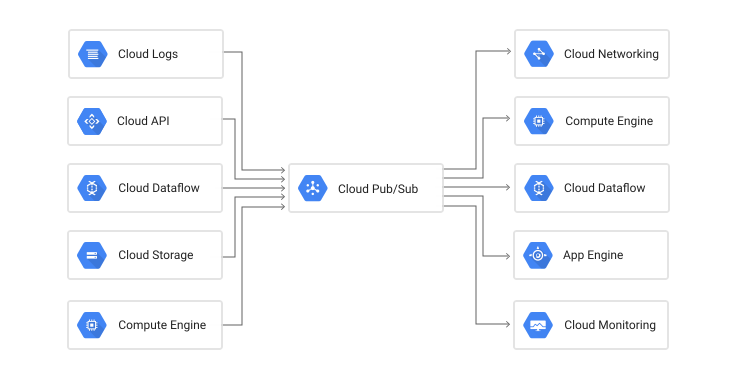
\includegraphics[width=\textwidth]{pubsub.png}
    \end{minipage}
};
\node[fancytitle, right=10pt] at (box.north west) {Pub/Sub};
\end{tikzpicture}





% ------------ ML Engine -----------------
\begin{tikzpicture}
\node [mybox] (box){%
    \begin{minipage}{0.3\textwidth}
    \setlist{nolistsep}	
   
    Managed infrastructure of GCP with the power and flexibility of TensorFlow. Can use it to train ML models at scale and host trained models to make predictions about new data in the cloud. Supported frameworks include Tensorflow, scikit-learn and XGBoost.\\
    
    {\color{blue} \textbf{ML Workflow}}\\
    Evaluate Problem: What is the problem and is ML the best approach? How will you measure model's success?\\ 
    \textbf{Choosing Development Environment}: Supports Python 2 and 3 and supports TF, scikit-learn, XGBoost as frameworks.\\
    \textbf{Data Preparation and Exploration}: Involves gathering, cleaning, transforming, exploring, splitting, and preprocessing data. Also includes feature engineering. \\ 
    \textbf{Model Training/Testing}: Provide access to train/test data and train them in batches. Evaluate progress/results and adjust the model as needed. Export/save trained model (250 MB or smaller to deploy in ML Engine).\\
    \textbf{Hyperparameter Tuning}: hyperparameters are variables that govern the training process itself, not related to the training data itself. Usually constant during training.\\
    \textbf{Prediction}: host your trained ML models in the cloud and use the Cloud ML prediction service to infer target values for new data\\
    
    {\color{blue} \textbf{ML APIs}}\\
    \textbf{Speech-to-Text}: speech-to-text conversion\\
    \textbf{Text-to-Speech}: text-to-speech conversion \\
    \textbf{Translation}: dynamically translate between languages\\
    \textbf{Vision}: derive insight (objects/text) from images\\
    \textbf{Natural Language}: extract information (sentiment, intent, entity, and syntax) about the text: people, places..\\
    \textbf{Video Intelligence}: extract metadata from videos\\
    
    {\color{blue} \textbf{Cloud Datalab}}\\
    Interactive tool (run on an instance) to explore, analyze, transform and visualize data and build machine learning models. Built on Jupyter. Datalab is free but may incus costs based on usages of other services.\\
    
    {\color{blue} \textbf{Data Studio}}\\
    Turns your data into informative dashboards and reports. Updates to data will automatiaclly update in dashbaord. \textbf{Query cache} remembers the queries (requests for data) issued by the components in a report (lightning bolt)- turn off for data that changes frequently, want to prioritize freshness over performance, or using a data source that incurs usage costs (e.g. BigQuery). \textbf{Prefetch cache} predicts data that could be requested by analyzing the dimensions, metrics, filters, and date range properties and controls on the report.

    \end{minipage}
};
\node[fancytitle, right=10pt] at (box.north west) {ML Engine};
\end{tikzpicture}


% ------------ ML Concepts/Terminology -----------------
\begin{tikzpicture}
\node [mybox] (box){%
    \begin{minipage}{0.3\textwidth}
    \setlist{nolistsep}	
	{\color{cyan} \textbf{Features}}: input data used by the ML model\\ 
    {\color{cyan}\textbf{Feature Engineering}}: transforming input features to be more useful for the models. e.g. mapping categories to buckets, normalizing between -1 and 1, removing null\\ 
   	{\color{cyan}\textbf{Train/Eval/Test}}: training is data used to optimize the model, evaluation is used to asses the model on new data during training, test is used to provide the final result\\ 	
    {\color{cyan}\textbf{Classification/Regression}}: regression is prediction a number (e.g. housing price), classification is prediction from a set of categories(e.g. predicting red/blue/green)\\
    {\color{cyan}\textbf{Linear Regression}}: predicts an output by multiplying and summing input features with weights and biases\\
    {\color{cyan}\textbf{Logistic Regression}}: similar to linear regression but predicts a probability\\
    {\color{cyan}\textbf{Neural Network}}: composed of neurons (simple building blocks that actually “learn”), contains activation functions that makes it possible to predict non-linear outputs\\
    {\color{cyan}\textbf{Activation Functions}}: mathematical functions that introduce non-linearity to a network e.g. RELU, tanh\\
    {\color{cyan}\textbf{Sigmoid Function}}: function that maps very negative numbers to a number very close to 0, huge numbers close to 1, and 0 to .5. Useful for predicting probabilities\\
    {\color{cyan}\textbf{Gradient Descent/Backpropagation}}: fundamental loss optimizer algorithms, of which the other optimizers are usually based. Backpropagation is similar to gradient descent but for neural nets \\
    {\color{cyan}\textbf{Optimizer}}: operation that changes the weights and biases to reduce loss e.g. Adagrad or Adam\\
    {\color{cyan}\textbf{Weights / Biases}}: weights are values that the input features are multiplied by to predict an output value. Biases are the value of the output given a weight of 0. \\
    {\color{cyan}\textbf{Converge}}: algorithm that converges will eventually reach an optimal answer, even if very slowly. An algorithm that doesn’t converge may never reach an optimal answer. \\
    {\color{cyan}\textbf{Learning Rate}}: rate at which optimizers change weights and biases. High learning rate generally trains faster but risks not converging, whereas a lower rate trains slower \\
    {\color{cyan}\textbf{Overfitting}}: model performs great on the input data but poorly on the test data (combat by dropout, early stopping, or reduce \# of nodes or layers)\\
    {\color{cyan}\textbf{Bias/Variance}}: how much output is determined by the features. more variance often can mean overfitting, more bias can mean a bad model \\
    {\color{cyan}\textbf{Regularization}}: variety of approaches to reduce overfitting, including adding the weights to the loss function, randomly dropping layers (dropout)\\
    {\color{cyan}\textbf{Ensemble Learning}}: training multiple models with different parameters to solve the same problem \\
%     {\color{cyan}\textbf{Numerical Instability}}: issues with very large/small values due to the limits of floating point numbers in computers\\
    {\color{cyan}\textbf{Embeddings}}: mapping from discrete objects, such as words, to vectors of real numbers. useful because classifiers/neural networks work well on vectors of real numbers
    
    \end{minipage}
};

\node[fancytitle, right=10pt] at (box.north west) {ML Concepts/Terminology};
\end{tikzpicture}



% ------------ TensorFlow -----------------
\begin{tikzpicture}
\node [mybox] (box){%
    \begin{minipage}{0.3\textwidth}
    \setlist{nolistsep}	
    
    
    Tensorflow is an open source software library for numerical computation using data flow graphs. Everything in TF is a graph, where nodes represent operations on data and edges represent the data. Phase 1 of TF is building up a computation graph and phase 2 is executing it. It is also distributed, meaning it can run on either a cluster of machines or just a single machine.  \\
    
    
    {\color{blue} \textbf{Tensors}}\\
    In a graph, tensors are the edges and are multidimensional data arrays that flow through the graph. Central unit of data in TF and consists of a set of primitive values shaped into an array of any number of dimensions.\\
    
    A tensor is characterized by its rank (\# dimensions in tensor), shape (\# of dimensions and size of each dimension), data type (data type of each element in tensor).\\
    
    {\color{blue} \textbf{Placeholders and Variables}}\\
    \textbf{Variables}: best way to represent shared, persistent state manipulated by your program. These are the parameters of the ML model are altered/trained during the training process. Training variables. \\
    \textbf{Placeholders}: way to specify inputs into a graph that hold the place for a Tensor that will be fed at runtime. They are assigned once, do not change after. Input nodes\\
    
    {\color{blue} \textbf{Popular Architectures}}\\
    \textbf{Linear Classifier}: takes input features and combines them with weights and biases to predict output value\\
	\textbf{DNNClassifier}: deep neural net, contains intermediate layers of nodes that represent “hidden features” and activation functions to represent non-linearity\\ 
    \textbf{ConvNets}: convolutional neural nets. popular for image classification. \\
    \textbf{Transfer Learning}: use existing trained models as starting points and add additional layers for the specific use case. idea is that highly trained existing models know general features that serve as a good starting point for training a small network on specific examples \\
    \textbf{RNN}: recurrent neural nets, designed for handling a sequence of inputs that have “memory” of the sequence. LSTMs are a fancy version of RNNs, popular for NLP
    \textbf{GAN}: general adversarial neural net, one model creates fake examples, and another model is served both fake example and real examples and is asked to distinguish\\
    \textbf{Wide and Deep}: combines linear classifiers with deep neural net classifiers, "wide" linear parts represent memorizing specific examples and “deep” parts represent understanding high level features\\



%     In ML, feature vectors are inputs/attributes which the ML algorithm focuses on. Each data point is a list (vector) of such vectors: aka feature vector. The output is a label or number.\\
%     Deep Learning is a representation ML based system that figures out by themselves what features to focus on. Neural networks are the most common class of deep learning algorithms, which are composed of neurons.
    \end{minipage}
};
\node[fancytitle, right=10pt] at (box.north west) {TensorFlow};
\end{tikzpicture}


% ------------ Case Study: Flowlogistic I-----------------
\begin{tikzpicture}
\node [mybox] (box){%
    \begin{minipage}{0.3\textwidth}
    \setlist{nolistsep}	

    {\color{blue} \textbf{Company Overview}}\\
    Flowlogistic is a top logistics and supply chain provider. They help businesses throughout the world manage their resources and transport them to their final destination. The company has grown rapidly, expanding their offerings to include rail, truck, aircraft, and oceanic shipping.\\
    
    {\color{blue} \textbf{Company Background}}\\
	The company started as a regional trucking company, and then expanded into other logistics markets. Because they have not updated their infrastructure, managing and tracking orders and shipments has become a bottleneck. To improve operations, Flowlogistic developed proprietary technology for tracking shipments in real time at the parcel level. However, they are unable to deploy it because their technology stack, based on Apache Kafka, cannot support the processing volume. In addition, Flowlogistic wants to further analyze their orders and shipments to determine how best to deploy their resources.\\
    
    {\color{blue} \textbf{Solution Concept}}\\
	Flowlogistic wants to implement two concepts in the cloud:  
    \begin{itemize}
    	\item Use their proprietary technology in a real-time inventory-tracking system that indicates the location of their loads.
        \item Perform analytics on all their orders and shipment logs (structured and unstructured data) to determine how best to deploy resources, which customers to target, and which markets to expand into. They also want to use predictive analytics to learn earlier when a shipment will be delayed.\\
	\end{itemize}
    
    {\color{blue} \textbf{Business Requirements}}\\
	-Build a reliable and reproducible environment with scaled parity of production\\
	-Aggregate data in a centralized Data Lake for analysis\\
	-Perform predictive analytics on future shipments\\
	-Accurately track every shipment worldwide\\
	-Improve business agility and speed of innovation through rapid provisioning of new resources\\
	-Analyze/optimize architecture cloud performance\\
	-Migrate fully to the cloud if all other requirements met \\
    
    {\color{blue} \textbf{ Technical Requirements}}\\
    -Handle both streaming and batch data\\
    -Migrate existing Hadoop workloads\\
    -Ensure architecture is scalable and elastic to meet the changing demands of the company\\
    -Use managed services whenever possible\\
    -Encrypt data in flight and at rest\\
    -Connect a VPN between the production data center and cloud environment
    \end{minipage}
};
\node[fancytitle, right=10pt] at (box.north west) {Case Study: Flowlogistic I};
\end{tikzpicture}

% ------------ Case Study: Flowlogistic II -----------------
\begin{tikzpicture}
\node [mybox] (box){%
    \begin{minipage}{0.3\textwidth}
    \setlist{nolistsep}	

    {\color{blue} \textbf{Existing Technical Environment}}\\
    Flowlogistic architecture resides in a single data center:
    \begin{itemize}
    	
		\item Databases:
          \begin{itemize}
              \item 8 physical servers in 2 clusters
              \begin{itemize}
                  \item SQL Server: inventory, user/static data
              \end{itemize}
              \item 3 physical servers
              \begin{itemize}
                  \item Cassandra: metadata, tracking messages
              \end{itemize}
              \item 10 Kafka servers: tracking message aggregation and batch insert
          \end{itemize}
        
        \item Application servers: customer front end, middleware for order/customs
         \begin{itemize}
         	\item 60 virtual machines across 20 physical servers
            \begin{itemize}
                \item Tomcat: Java services
                \item Nginx: static content
                \item Batch servers
            \end{itemize}
          \end{itemize}
        
        \item Storage appliances
        	\begin{itemize}
                \item iSCSI for virtual machine (VM) hosts
                \item Fibre Channel storage area network (FC SAN): SQL server storage

                \item Network-attached storage (NAS): image storage, logs, backups

            \end{itemize}
       \item 10 Apache Hadoop / Spark Servers
          \begin{itemize}
              \item Core Data Lake
              \item Data analysis workloads
          \end{itemize}
          
       \item 20 miscellaneous servers
       		\begin{itemize}
              \item Jenkins, monitoring, bastion hosts, security scanners, billing software\\
            \end{itemize}
	\end{itemize}
    
    {\color{blue} \textbf{CEO Statement}}\\
    We have grown so quickly that our inability to upgrade our infrastructure is really hampering further growth/efficiency. We are efficient at moving shipments around the world, but we are inefficient at moving data around. We need to organize our information so we can more easily understand where our customers are and what they are shipping.\\
    
    {\color{blue} \textbf{CTO Statement}}\\
    IT has never been a priority for us, so as our data has grown, we have not invested enough in our technology. I have a good staff to manage IT, but they are so busy managing our infrastructure that I cannot get them to do the things that really matter, such as organizing our data, building the analytics, and figuring out how to implement the CFO’s tracking technology.\\

    {\color{blue} \textbf{CFO Statement}}\\
    Part of our competitive advantage is that we penalize ourselves for late shipments/deliveries. Knowing where our shipments are at all times has a direct correlation to our bottom line and profitability. Additionally, I don’t want to commit capital to building out a server environment.
    \end{minipage}
};
\node[fancytitle, right=10pt] at (box.north west) {Case Study: Flowlogistic II};
\end{tikzpicture}


% ------------ Flowlogistic Potential Solution -----------------
\begin{tikzpicture}
\node [mybox] (box){%
    \begin{minipage}{0.3\textwidth}
    \setlist{nolistsep}	

    \begin{enumerate}
     	\item Cloud Dataproc handles the existing workloads and produces results as before (using a VPN).
    	\item At the same time, data is received through the data center, via either stream or batch, and sent to Pub/Sub.
        \item Pub/Sub encrypts the data in transit and at rest.
        \item Data is fed into Dataflow either as stream/batch data.
        \item Dataflow processes the data and sends the cleaned data to BigQuery (again either as stream or batch).
        \item Data can then be queried from BigQuery and predictive analysis can begin (using ML Engine, etc..) 
	\end{enumerate}   	 
    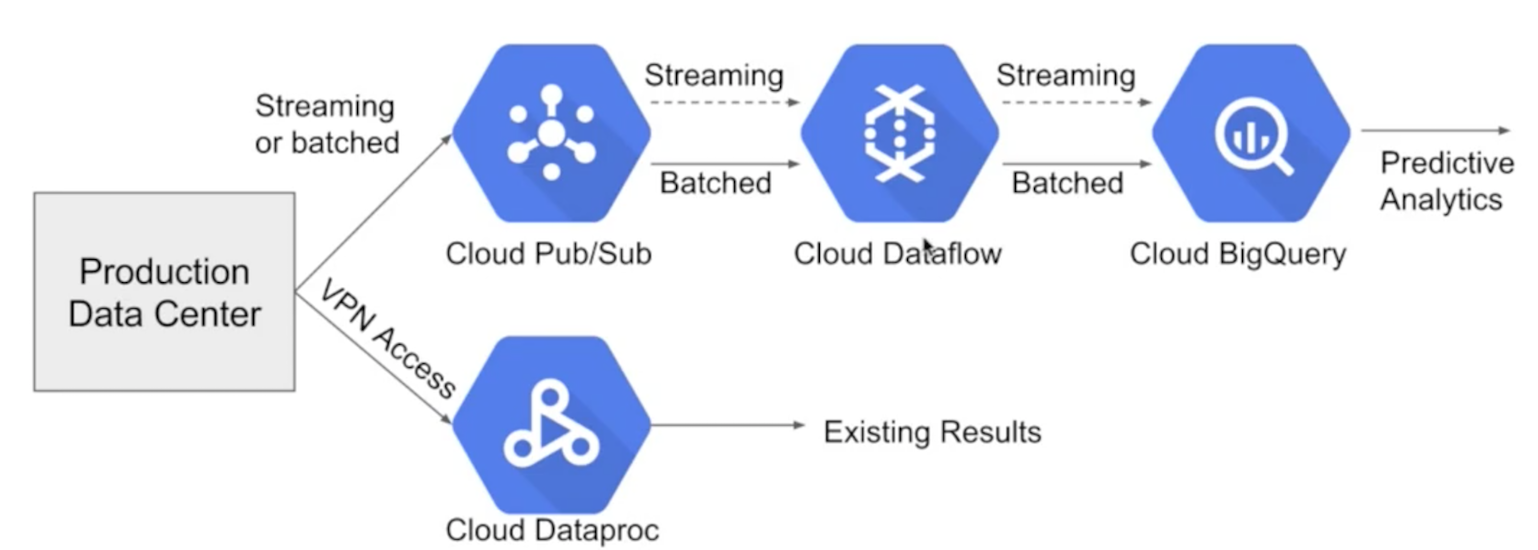
\includegraphics[width=\textwidth]{Figures/flowlogistic_sol.png}
    \textbf{\textit{Note}}: All services are fully managed., easily scalable, and can handle streaming/batch data. All technical requirements are met.

    \end{minipage}
};
\node[fancytitle, right=10pt] at (box.north west) {Flowlogistic Potential Solution};
\end{tikzpicture}

% ------------ MJTelco Case Study I -----------------
\begin{tikzpicture}
\node [mybox] (box){%
    \begin{minipage}{0.3\textwidth}
    \setlist{nolistsep}	

    {\color{blue} \textbf{Company Overview}}\\
    MJTelco is a startup that plans to build networks in rapidly growing, underserved markets around the world. The company has patents for innovative optical communications hardware. Based on these patents, they can create many reliable, high-speed backbone links with inexpensive hardware.\\

	{\color{blue} \textbf{Company Background}}\\
    Founded by experienced telecom executives, MJTelco uses technologies originally developed to overcome communications challenges in space. Fundamental to their operation, they need to create a distributed data infrastructure that drives real-time analysis and incorporates machine learning to continuously optimize their topologies. Because their hardware is inexpensive, they plan to overdeploy the network allowing them to account for the impact of dynamic regional politics on location availability and cost.\\
    
    Their management and operations teams are situated all around the globe creating many-to-many relationship between data consumers and providers in their system. After careful consideration, they decided public cloud is the perfect environment to support their needs.\\
    
    {\color{blue} \textbf{Solution Concept}}\\
    MJTelco is running a successful proof-of-concept (PoC) project in its labs. They have two primary needs:
	\begin{itemize}
		\item Scale and harden their PoC to support significantly more data flows generated when they ramp to more than 50,000 installations.
		\item Refine their machine-learning cycles to verify and improve the dynamic models they use to control topology definitions.
MJTelco will also use three separate operating environments -- development/test, staging, and production -- to meet the needs of running experiments, deploying new features, and serving production customers.\\
	\end{itemize}

    {\color{blue} \textbf{Business Requirements}}\\
    -Scale up their production environment with minimal cost, instantiating resources when and where needed in an unpredictable, distributed telecom user community.\\
    -Ensure security of their proprietary data to protect their leading-edge machine learning and analysis.\\
    -Provide reliable and timely access to data for analysis from distributed research workers.\\
    -Maintain isolated environments that support rapid iteration of their machine-learning models without affecting their customers.
   
    \end{minipage}
};
\node[fancytitle, right=10pt] at (box.north west) {Case Study: MJTelco I};
\end{tikzpicture}

% ------------ Case Study: MJTelco II -----------------
\begin{tikzpicture}
\node [mybox] (box){%
    \begin{minipage}{0.3\textwidth}
    \setlist{nolistsep}	

    {\color{blue} \textbf{Technical Requirements}}\\
    -Ensure secure and efficient transport and storage of telemetry data.\\
    -Rapidly scale instances to support between 10,000 and 100,000 data providers with multiple flows each.\\
    -Allow analysis and presentation against data tables tracking up to 2 years of data storing approximately 100m records/day.
Support rapid iteration of monitoring infrastructure focused on awareness of data pipeline problems both in telemetry flows and in production learning cycles.\\

    {\color{blue} \textbf{CEO Statement}}\\
    Our business model relies on our patents, analytics and dynamic machine learning. Our inexpensive hardware is organized to be highly reliable, which gives us cost advantages. We need to quickly stabilize our large distributed data pipelines to meet our reliability and capacity commitments.\\

    {\color{blue} \textbf{CTO Statement}}\\
Our public cloud services must operate as advertised. We need resources that scale and keep our data secure. We also need environments in which our data scientists can carefully study and quickly adapt our models. Because we rely on automation to process our data, we also need our development and test environments to work as we iterate.\\

    {\color{blue} \textbf{CFO Statement}}\\
This project is too large for us to maintain the hardware and software required for the data and analysis. Also, we cannot afford to staff an operations team to monitor so many data feeds, so we will rely on automation and infrastructure. Google Cloud’s machine learning will allow our quantitative researchers to work on our high-value problems instead of problems with our data pipelines.
    \end{minipage}
};
\node[fancytitle, right=10pt] at (box.north west) {Case Study: MJTelco II};
\end{tikzpicture}


% ------------ Choosing a Storage Option -----------------
\begin{tikzpicture}
\node [mybox] (box){%
    \begin{minipage}{0.3\textwidth}
    \setlist{nolistsep}	
    
    \begin{tabularx}{\textwidth}{X|p{2.4cm}|p{2.4cm}}
      \textbf{Need} & \textbf{Open Source} & \textbf{GCP Solution} \\
    \hline
    Compute, Block Storage & Persistent Disks, SSD & Persistent Disks, SSD\\
    \hline
    Media, Blob Storage & Filesystem, HDFS & Cloud Storage\\
    \hline
    SQL Interface on File Data & Hive & BigQuery\\
    \hline
    Document DB, NoSQL & CouchDB, MongoDB & DataStore\\
    \hline    
    Fast Scanning NoSQL & HBase, Cassandra & BigTable\\
    \hline    
    OLTP & RDBMS- MySQL & CloudSQL, Cloud Spanner\\
    \hline
    OLAP & Hive & BigQuery\\
    \hline
    \end{tabularx}
    
    \textbf{Cloud Storage}: unstructured data (blob)\\
%     Cloud Storage for Firebase: unstructured data (blob), need for mobile SDKs\\
    \textbf{CloudSQL}: OLTP, SQL, structured and relational data, no need for horizontal scaling\\
    \textbf{Cloud Spanner}: OLTP, SQL, structured and relational data, need for horizontal scaling, between RDBMS/big data\\
    \textbf{Cloud Datastore}: NoSQL, document data, key-value structured but non-relational data (XML, HTML, query depends on size of result (not dataset), fast to read/slow to write\\
    \textbf{BigTable}: NoSQL, key-value data, columnar, good for sparse data, sensitive to hot spotting, high throughput and scalability for non-structured key/value data, where each value is typically no larger than 10 MB  

    \end{minipage}
};
\node[fancytitle, right=10pt] at (box.north west) {Choosing a Storage Option};
\end{tikzpicture}


% ------------ Solutions -----------------
\begin{tikzpicture}
\node [mybox] (box){%
    \begin{minipage}{0.3\textwidth}
    \setlist{nolistsep}	

    {\color{blue} \textbf{Data Lifecycle}}\\
    At each stage, GCP offers multiple services to manage your data.
    \begin{enumerate}
    	\item \textbf{Ingest}: first stage is to pull in the raw data, such as streaming data from devices, on-premises batch data, application logs, or mobile-app user events and analytics
        \item \textbf{Store}: after the data has been retrieved, it needs to be stored in a format that is durable and can be easily accessed
        \item \textbf{Process and Analyze}: the data is transformed from raw form into actionable information
        \item \textbf{Explore and Visualize}: convert the results of the analysis into a format that is easy to draw insights from and to share with colleagues and peers
	\end{enumerate}
    
    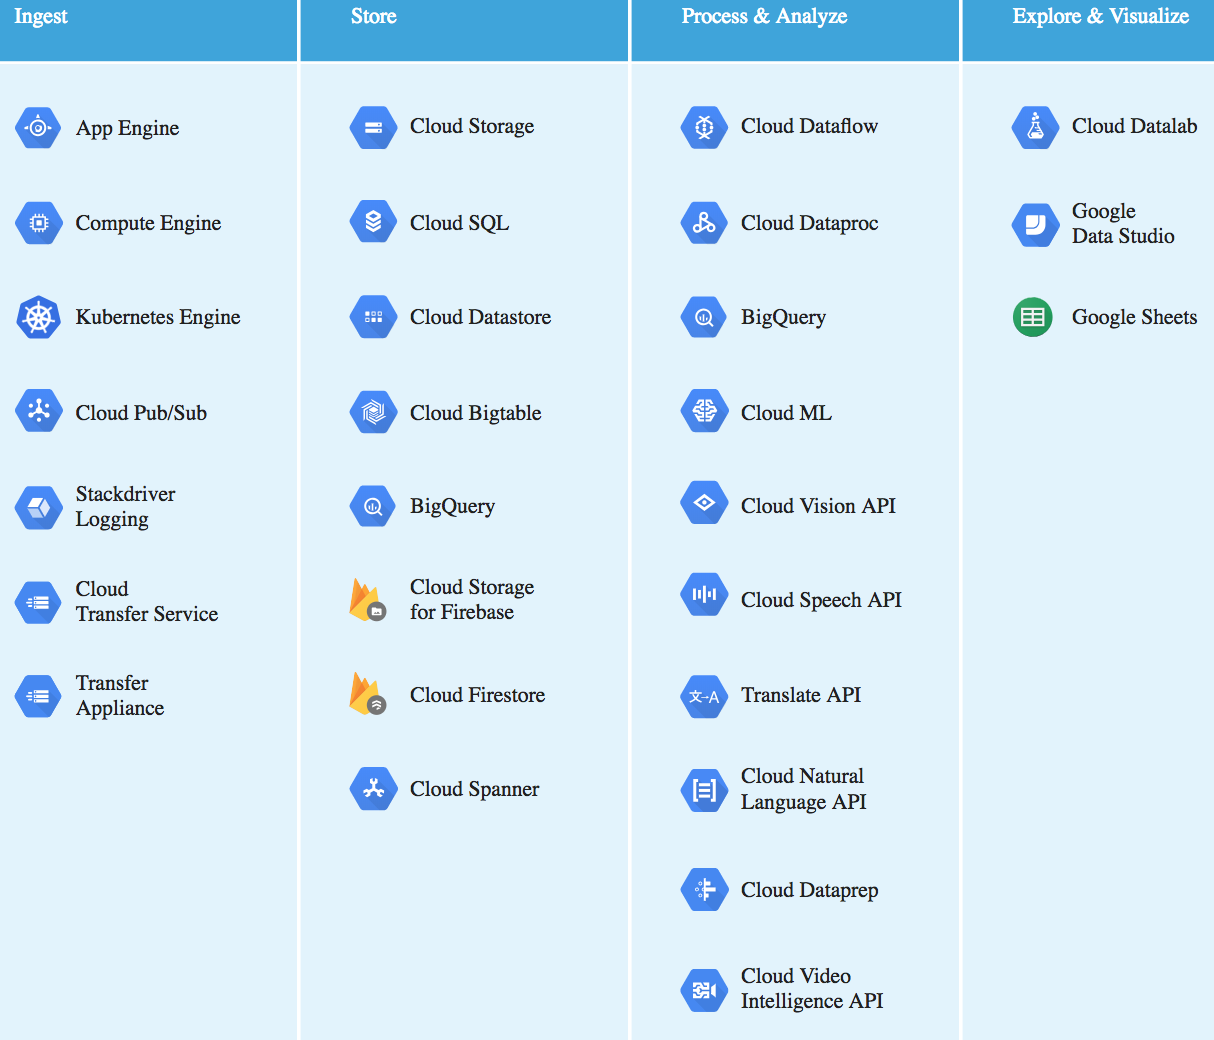
\includegraphics[width=\textwidth]{Figures/Data_Lifecycle_Solutions.png}
   

    {\color{blue} \textbf{Ingest}}\\
    There are a number of approaches to collect raw data, based on the data’s size, source, and latency.
    \begin{itemize}
    	\item \textbf{Application}: data from application events, log files or user events, typically collected in a push model, where the application calls an API to send the data to storage (Stackdriver Logging, Pub/Sub, CloudSQL, Datastore, Bigtable, Spanner)
        \item \textbf{Streaming}: data consists of a continuous stream of small, asynchronous messages. Common uses include telemetry, or collecting data from geographically dispersed devices (IoT) and user events and analytics (Pub/Sub)
        \item  \textbf{Batch}: large amounts of data are stored in a set of files that are transferred to storage in bulk. common use cases include scientific workloads, backups, migration (Storage, Transfer Service, Appliance)
    \end{itemize}

    \end{minipage}
};
\node[fancytitle, right=10pt] at (box.north west) {Solutions};
\end{tikzpicture}

% ------------ SOlutions Part II -----------------
\begin{tikzpicture}
\node [mybox] (box){%
    \begin{minipage}{0.3\textwidth}
    \setlist{nolistsep}	

    {\color{blue} \textbf{Storage}}\\
    \textbf{Cloud Storage}: durable and highly-available object storage for structured and unstructured data\\
    \textbf{Cloud SQL}: fully managed, cloud RDBMS that offers both MySQL and PostgreSQL engines with built-in support for replication, for low-latency, transactional, relational database workloads. supports RDBMS workloads up to 10 TB (storing financial transactions, user credentials, customer orders)\\
    \textbf{BigTable}: managed, high-performance NoSQL database service designed for terabyte- to petabyte-scale workloads. suitable for large-scale, high-throughput workloads such as advertising technology or IoT data infrastructure. does not support multi-row transactions, SQL queries or joins, consider Cloud SQL or Cloud Datastore instead\\
    \textbf{Cloud Spanner}: fully managed relational database service for mission-critical OLTP applications. horizontally scalable, and built for strong consistency, high availability, and global scale. supports schemas, ACID transactions, and SQL queries (use for retail and global supply chain, ad tech, financial services)\\
    \textbf{BigQuery}: stores large quantities of data for query and analysis instead of transactional processing
    
    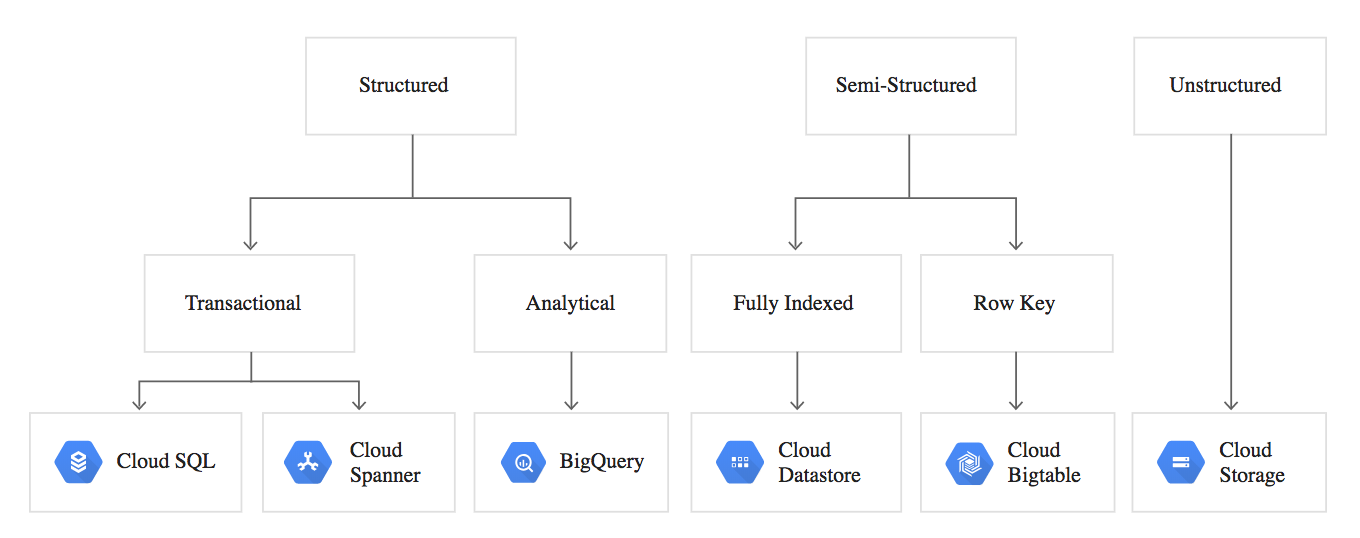
\includegraphics[width=\textwidth]{Figures/Solutions-_Storage.png}\\

    {\color{blue} \textbf{Exploration and Visualization}}
    Data exploration and visualization to better understand the results of the processing and analysis.
    \begin{itemize}
    	\item \textbf{Cloud Datalab}: interactive web-based tool that you can use to explore, analyze and visualize data built on top of Jupyter notebooks. runs on a VM and automatically saved to persistent disks and can be stored in GC Source Repo (git repo)
        \item \textbf{Data Studio}: drag-and-drop report builder that you can use to visualize data into reports and dashboards that can then be shared with others, backed by live data, that can be shared and updated easily. data sources can be data files, Google Sheets, Cloud SQL, and BigQuery. supports \textbf{query} and \textbf{prefetch cache}: query remembers previous queries and if data not found, goes to prefetch cache, which predicts data that could be requested (disable if data changes frequently/using data source incurs charges)
    \end{itemize}




    \end{minipage}
};
\node[fancytitle, right=10pt] at (box.north west) {Solutions- Part II};
\end{tikzpicture}

% ------------ TEMPLATE -----------------
\begin{tikzpicture}
\node [mybox] (box){%
    \begin{minipage}{0.3\textwidth}
    \setlist{nolistsep}	

     {\color{blue} \textbf{Process and Analyze}}\\
    In order to derive business value and insights from data, you must transform and analyze it. This requires a processing framework that can either analyze the data directly or prepare the data for downstream analysis, as well as tools to analyze and understand processing results.
    \begin{itemize}
    	\item \textbf{Processing}: data from source systems is cleansed, normalized, and processed across multiple machines, and stored in analytical systems
        \item \textbf{Analysis}: processed data is stored in systems that allow for ad-hoc querying and exploration
        \item \textbf{Understanding}: based on analytical results, data is used to train and test automated machine-learning models
	\end{itemize}
       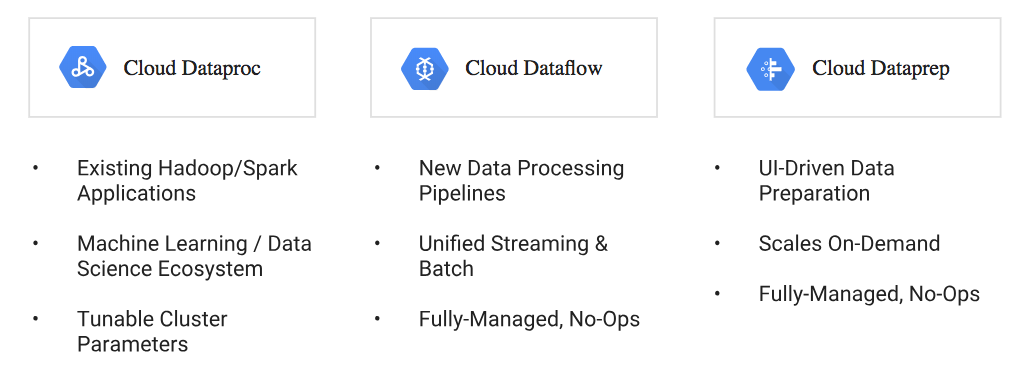
\includegraphics[width=\textwidth]{Figures/Solutions-_Proces_Analyze.png}
       
    {\color{cyan} \textbf{Processing}}
    \begin{itemize}
    \item \textbf{Cloud Dataproc}: migrate your existing Hadoop or Spark deployments to a fully-managed service that automates cluster creation, simplifies configuration and management of your cluster, has built-in monitoring and utilization reports, and can be shutdown when not in use
    \item\textbf{Cloud Dataflow}: designed to simplify big data for both streaming and batch workloads, focus on filtering, aggregating, and transforming your data
    \item\textbf{Cloud Dataprep}: service for visually exploring, cleaning, and preparing data for analysis. can transform data of any size stored in CSV, JSON, or relational-table formats\\
    \end{itemize}
    
    {\color{cyan} \textbf{Analyzing and Querying}}
    \begin{itemize}
    \item \textbf{BigQuery}: query using SQL, all data encrypted, user analysis, device and operational metrics, business intelligence
    \item \textbf{Task-Specific ML}: Vision, Speech, Natural Language, Translation, Video Intelligence
    \item \textbf{ML Engine}: managed platform you can use to run custom machine learning models at scale
    \end{itemize}

    
    \end{minipage}
};
\node[fancytitle, right=10pt] at (box.north west) {Solutions- Part III};
\end{tikzpicture}


streaming data: use Pub/Sub and Dataflow in combination


    

% % ------------------------------------------------------------------------
% % ------------ TEMPLATE -----------------
% \begin{tikzpicture}
% \node [mybox] (box){%
%     \begin{minipage}{0.3\textwidth}
%     \setlist{nolistsep}	

%     {\color{blue} \textbf{TEMPLATE}}\\
    
%     \begin{itemize}
%     	\item
% 	\end{itemize}
%     \end{minipage}
% };
% \node[fancytitle, right=10pt] at (box.north west) {TEMPLATE};
% \end{tikzpicture}
% % ------------------------------------------------------------------------

\end{multicols*}
\end{document}
Contact GitHub API Training Shop Blog About
© 2016 GitHub, Inc. Terms Privacy Security Status Help